\documentclass[draft]{beamer}
%%%%%%%%%%%%%%%%%%%%%%%%%%%%%%%%%%%%%%%%%%%%%%%%%%%%%%%%%%%%%%%%%%%%%%%%%%%%
\usepackage{bm}
\usepackage{amsmath}
\usepackage{amssymb}
%\usepackage{microtype}
\usepackage{booktabs} % \toprule, \midrule, \bottomrule
%%% INCLUDE FILE FOR DEFINITIONS
%%% These may require various packages.

% Shortcuts in regular text
\newcommand{\degs}{\ensuremath{^\circ}}
\newcommand{\EE}[1]{\ensuremath{\times 10^{#1}}}
\newcommand{\ttimes}{\ensuremath{{}\times{}}}
\newcommand{\cclicense}{%
  \smash{\raisebox{-0.45ex}{%
  \setlength{\unitlength}{1em}%
  \begin{picture}(1,1)%
    \put(0.5,0.5){\circle{1}}
    \put(0.5,0.5){\hbox to 0pt{\hss\raisebox{-.45ex}{\tiny\textsf{CC}}\hss}}
  \end{picture}%
  }}%
  \hskip -1em%
  \href{http://creativecommons.org/licenses/by-nc-sa/3.0/}%
  {\ \hskip 1em \textsf{BY-NC-SA}}%
}

%\newcommand{\horizsep}{{\par\noindent\centering\rule[.25ex]{.75\columnwidth}{2pt}\par}}
\newcommand{\horizsep}{\vspace{\baselineskip}\noindent\hspace{\stretch{1}}$
\ast\qquad \ast\qquad \ast\qquad
$ \hspace{\stretch{1}} \vspace{\baselineskip}}
\newcommand{\pytrt}{\textsf{PyTRT}}

% Research
\newcommand{\lop}[1]{\mathcal{L}\!\left[#1\right]}
\newcommand{\lopinv}[2]{\mathcal{I}_{#1}\!\left[#2\right]}
\newcommand{\Dtens}{\mat{D}}
\newcommand{\Etens}{\mat{E}}
\newcommand{\Identitytens}{\mat{I}}
\newcommand{\APone}{AP$_1$}
\newcommand{\Pone}{P$_1$}
\newcommand{\SN}{S$_N$}%{S$_\text{N}$}%{$S_N$}%
\newcommand{\PN}{P$_N$}%{P$_\text{N}$}%{$P_N$}%
\newcommand{\CN}{Crank--Nicolson} %Yes, it's Nic not Nich
\newcommand{\Eddington}{\mathcal{E}} %whatever symbol I decided for Eddington
\newcommand{\RadEn}{E} %whatever symbol I decide for radiation energy
\newcommand{\Sigmatr}{\Sigma_{\mathit{tr}}}

% Program names
\newcommand{\cpp}{\textsf{C\raisebox{0.2ex}{++}}}

% General math shortcuts
\newcommand{\ud}{\mathop{}\!\mathrm{d}}
\newcommand{\pder}[2]{\frac{\partial #1}{\partial #2}}
\newcommand{\oder}[2]{\frac{\mathrm{d} #1}{\mathrm{d} #2}}
\newcommand{\tpder}[2]{{\partial #1}/{\partial #2}} %inlined
\newcommand{\toder}[2]{{\mathrm{d} #1}/{\mathrm{d} #2}} %inlined
\newcommand{\lra}{ \quad \Longrightarrow \quad }
\newcommand{\eexp}{\mathop{}\!\mathrm{e}} % upright ``e'' for exponent
\newcommand{\expp}[1]{\exp\!\left( {#1} \right)} % exp with parentheses
\newcommand{\qeq}{\stackrel{\mathrm{?}}{=}}

% Probability
\newcommand{\expectation}[1]{\mathop{}\!\mathrm{E}\!\left[ #1 \right]}
\DeclareMathOperator{\Var}{Var} % variance

% Asymptotic analysis
\DeclareMathOperator{\Ei}{Ei} % Exponential function
\newcommand{\lapl}[1]{\mathcal{L}[{#1}]} %laplace

%change the Re and Im operators from fancy curly letters
\DeclareMathOperator{\MathOpRe}{Re}
\renewcommand{\Re}{\MathOpRe}
\DeclareMathOperator{\MathOpIm}{Im}
\renewcommand{\Im}{\MathOpIm}

%imaginary ``i'' , upright 'i' or \imath
\newcommand{\iimag}{\mathrm{i}}

% Finite differences
\newcommand{\hot}{\text{h.o.t.}}
\newcommand{\inv}{^{-1}}

% Numerical Linear Algebra
\newcommand{\conj}{^{\ast}} % complex conjugate (transpose)
\newcommand{\norm}[1]{\left\| #1 \right\|} % double pipe
\newcommand{\abs}[1]{\left| #1 \right|} % single pipe
\newcommand{\eps}{\varepsilon}
\DeclareMathOperator{\fl}{fl}

\DeclareMathOperator{\acosh}{arccosh} 

% Define a command to write a nice-looking element, e.g. 4,2 He
\newcommand{\elem}[3]{\ensuremath{{}^{{#1}}_{{#2}}\mathrm{{#3}}}}

% Vector definitions
\newcommand{\mat}[1]{\mathbf{#1}} %matrix is bold upright
\renewcommand{\vec}[1]{\bm{#1}} %vector is bold italic
\newcommand{\op}[1]{\mathsf{#1}} % ``operator'' is sans serif

\newcommand{\vd}{\bm{\cdot}} % slightly bold vector dot
\newcommand{\del}{\vec{\nabla}} % gradient (Del) is bold
\newcommand{\grad}{\vec{\nabla}} % gradient

%\newcommand{\abr}[1]{\langle {#1} \rangle}
\newcommand{\abr}[1]{\left\langle {#1} \right\rangle} % angle brackets for avg.

%% topbox is useful in extended definitions of math terms inside an align
\newcommand{\topbox}[2][0.6]{\parbox[t]{#1\columnwidth}{\raggedright{}#2}}

% commands to make text in math mode appear as zero-width (better-looking
% integrals/sums, e.g.)
% from mathmode.pdf page 74, or Alexander R. Perlis ``A complement to \smash,
% \llap, and \rlap''

\def\mathllap{\mathpalette\mathllapinternal}
	\def\mathllapinternal#1#2{%
	\llap{$\mathsurround=0pt#1{#2}$}%
}
\def\clap#1{\hbox to 0pt{\hss#1\hss}}%
\def\mathclap{\mathpalette\mathclapinternal}%
\def\mathclapinternal#1#2{%
	\clap{$\mathsurround=0pt#1{#2}$}%
}
\def\mathrlap{\mathpalette\mathrlapinternal}%
\def\mathrlapinternal#1#2{%
	\rlap{$\mathsurround=0pt#1{#2}$}%
}

\definecolor{lightgray}{gray}{0.85}
%%%%%%%%%%%%%%%%%%%%%%%%%%%%%%%%%%%%%%%%%%%%%%%%%%%%%%%%%%%%%%%%%%%%%%%%%%%%

\usetheme{AnnArbor}
\usecolortheme{seahorse}
\usecolortheme{orchid}
\usefonttheme[onlymath]{serif}
\setbeamercolor*{frametitle}{use=structure,bg=structure.fg!20!white}
\setbeamercolor*{frametitle right}{use=structure,bg=structure.fg!20!white}
\setbeamertemplate{navigation symbols}{\insertframenavigationsymbol}
\setbeamertemplate{caption}[numbered]

\title[ORNL Seminar]%
{An anisotropic diffusion approximation to nonlinear radiation transport}
%\subtitle{}

\author[SRJ, EWL]{Seth~Johnson, Ed~Larsen}

\institute[UMich]{
University of Michigan, Ann Arbor
}
\date[5/6/2011]{May 6, 2011}

\AtBeginSection[]
{
\begin{frame}
  \frametitle{Outline}
  \tableofcontents[currentsection]
\end{frame}
}

\hypersetup{colorlinks=true,linkcolor=black}

% only show section headings in table of contents
\setcounter{tocdepth}{1}

%use symbols for footnote
\renewcommand{\thefootnote}{\fnsymbol{footnote}}

\begin{document}
%%%%%%%%%%%%%%%%%%%%%%%%%%%%%%%%%%%%%%%%%%%%%%%%%%%%%%%%%%%%%%%%%%%%%%%%%%%%

\begin{frame}
\titlepage
\begin{center}
  
\includegraphics[width=0.2\textwidth]{../figures/umlogo}
\end{center}
\end{frame}

%%%%%%%%%%%%%%%%%%%%%%%%%%%%%%%%%%%%%%%%%%%%%%%%%%%%%%%%%%%%%%%%%%%%%%%%%%%%
\section{Introduction}
%%%%%%%%%%%%%%%%%%%%%%%%%%%%%%%%%%%%%%%%
\begin{frame}
  \frametitle{Thermal radiative transfer}
  \begin{itemize}
    \item TRT is the dominant heat transfer process in very hot materials
    \item Photons born isotropically via black body emission
      ($q_\text{rad} \propto \sigma T^4$)
    \item Cold material heats up and becomes relatively transparent
      ($\sigma\propto T^{-3}$)
  \end{itemize}

  Difficulties in solving:
  \begin{itemize}
    \item High dimensionality of solution phase space $(\vec{x}, \vec{\Omega},
      h\nu, t)$
    \item Highly nonlinear coupled partial differential equations for radiation
      field $I(\vec{x}, \vec{\Omega}, h\nu, t)$ and material energy
  \end{itemize}

  Particular application of this work: CRASH project
  \begin{itemize}
    \item Center for RAdiative Shock Hydrodynamics program: ``Assessment
      of Predictive Capability''
    \item Simulate laser-driven shock in a xenon-filled tube
    \item Uncertainty quantification: hundreds of solution instances needed
  \end{itemize}
\end{frame}

%%%%%%%%%%%%%%%%%%%%%%%%%%%%%%%%%%%%%%%%
\begin{frame}
  \frametitle{Motivation}
\begin{center}
  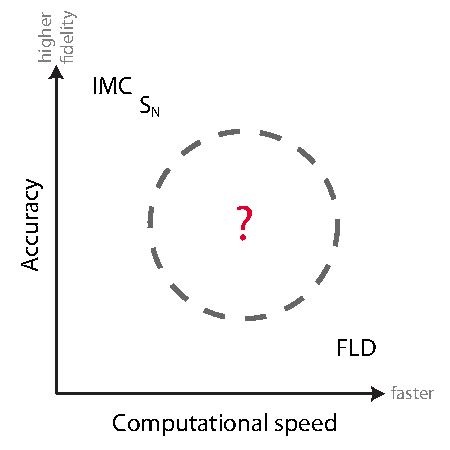
\includegraphics[width=3in]{../figures/fidelity}
\end{center}
% also, storage requirements
\end{frame}

%%%%%%%%%%%%%%%%%%%%%%%%%%%%%%%%%%%%%%%%
\begin{frame}
  \frametitle{Gray TRT equations}
  Common approximations for radiation transport methods development:
  \begin{itemize}
    \item work in a fixed medium, disregarding material advection;
    \item assume local thermodynamic equilibrium (LTE), which uses a single
      material temperature;
    \item neglect thermal conduction in material;
    \item average over all photon energies $h\nu$ (gray).
  \end{itemize}
\begin{subequations} \label{eqs:fullGrayTRT}
  Radiation transfer equation, intensity $I(\vec{x}, \vec{\Omega}, t)$:
\begin{equation} \label{eq:fullGrayTransport}
  \frac{1}{c} \pder{I}{t}
  + \vec{\Omega} \vd \del I +
 \sigma I
  = \frac{\sigma c aT^4}{4\pi} 
  + \frac{c Q}{4\pi}
\end{equation}
  Material energy balance equation:
\begin{equation} \label{eq:fullGrayMaterial}
  \frac{1}{c_v}\pder{T}{t} = \sigma \int_{4\pi}  I \ud \Omega - \sigma c aT^4
\end{equation}
\end{subequations}
\end{frame}

%%%%%%%%%%%%%%%%%%%%%%%%%%%%%%%%%%%%%%%%
\begin{frame}
  \frametitle{Anisotropic diffusion}
  Previous work:
  \begin{itemize}
    \item Steady-state infinite medium VHTR-like problem with analytically
      calculated coefficients \cite{Lar2009c}
    \item Non-local tensor diffusion \cite{Mor2007} for steady-state
      radiative transfer, no further development or analysis in literature
  \end{itemize}
  Current work:
  \begin{itemize}
    \item Formulates boundary conditions and time-dependent terms
    \item Uses transport-calculated anisotropic diffusion tensors
    \item Application to TRT problems
  \end{itemize}
  Potential applications:
  \begin{itemize}
    \item Extends diffusion theory to new regimes of applicability
    \item Variance reduction with shielding problems that have voids
  \end{itemize}
\end{frame}

%%%%%%%%%%%%%%%%%%%%%%%%%%%%%%%%%%%%%%%%%%%%%%%%%%%%%%%%%%%%%%%%%%%%%%%%%%%%
\section{Theory}
%%%%%%%%%%%%%%%%%%%%%%%%%%%%%%%%%%%%%%%%
\begin{frame}
  \frametitle{Summary in advance}
  \begin{enumerate}
    \item Start with time-dependent radiation transport equation with frozen
      opacities. Neglect $\frac{1}{c}\pder{I}{t}$ term to get anisotropic
      diffusion instead of anisotropic P$_1$.
    \item Multiply the zeroth moment of the transport equation by $1/4\pi$,
      subtract from the transport equation.
    \item Define $\Psi=I - \frac1{4\pi} \phi$, convert to an integral transport
      equation for $\Psi$ that has nonlocal unknowns.
    \item Use Taylor series to approximate nonlocal unknowns with local
      unknowns.
    \item Require that the contribution of boundary terms is zero: this gives
      boundary conditions for the new approximate method.
    \item Take the first angular moment of this new approximate angular
      intensity to get an approximate radiation flux.
    \item Substitute into time-dependent particle conservation equation to get
      time-dependent anisotropic diffusion.
  \end{enumerate}
%  \begin{enumerate}
%    \item Consider radiation transport equation $\lop{I}=\hat Q$ over a time
%      step, with opacities frozen at $\sigma^*$. Discard the time derivative
%      term and initial condition to get time-dependent anisotropic diffusion
%      instead of time-dependent \APone
%    \item Apply $\lopinv{}{\cdot}$ to convert the integrodifferential transport
%      equation to an integral transport equation along characteristic rays.
%    \item Average radiation transport equation over $\vec{\Omega}$, apply
%      $\lopinv{}{\cdot}$, subtract from integral equation for $I$
%    \item Apply Taylor series to non-local quantities $\phi$ to get an
%      approximate expression for $I(\vec{x}, \vec{\Omega})$ as a function of
%      $\phi(\vec{x})$ and other problem-dependent quantities.
%    \item Require that the boundary term disappears over the entire problem to
%      get boundary conditions
%    \item Take first moment of this approximate $I$ to get $\vec{F}(\vec{x})$,
%      which is used in time-dependent particle conservation equation.
%  \end{enumerate}
\end{frame}

\subsection{Anisotropic diffusion derivation}
%%%%%%%%%%%%%%%%%%%%%%%%%%%%%%%%%%%%%%%%
\begin{frame}%{Transport equation}
\begin{subequations} \label{eqs:fullTransport}
\begin{multline} \label{eq:fullTransportVol}
    \vec{\Omega}\vd \grad I(\vec{x}, \vec{\Omega})
    + \sigma^\ast(\vec{x}) I (\vec{x}, \vec{\Omega})
    = \frac{1}{4\pi} \sigma^\ast(\vec{x}) ac [T(\vec{x})]^4
    + \frac{1}{4\pi} q_{r}(\vec{x})
\\
    \equiv \frac{1}{4\pi} Q(\vec{x})
    \equiv \hat Q(\vec{x}, \vec{\Omega}) \,,
%\\
\quad
x \in V,\  \vec{\Omega} \in 4\pi,
\end{multline}
\begin{equation} \label{eq:fullTransportBndy}
  I(\vec{x}, \vec{\Omega}, t) = I^b(\vec{x}, \vec{\Omega}, t) \,,
 \quad \vec{x} \in \partial V, \ \vec{\Omega} \vd \vec{n} < 0.
\end{equation}
\end{subequations}
\begin{subequations} \label{eqs:inverseTransport}
  Integral transport equation \cite{Pri2010}:
  \begin{align} \label{eq:inverseTransportFull}
    I(\vec{x}, \vec{\Omega})
    &=
    I^b(\vec{x}_b, \vec{\Omega})
    \eexp^{ -\tau(\vec{x}, \vec{x}_b)}
    + \int_{0}^{\norm{\vec{x} - \vec{x}_b}}
    \left[ \hat Q(\vec{x} - s \vec{\Omega}, \vec{\Omega})
    \right]
    \eexp^{ -\tau(\vec{x}, \vec{x} - s \vec{\Omega})}
    \ud s
    \\ \label{eq:lopinv}
    &\equiv \lopinv{b}{I^b}
    + \lopinv{v}{\hat Q} 
  \end{align}
  Optical thickness: 
  \begin{equation} \label{eq:fullTauDefinition}
    \tau(\vec{x}, \vec{x}') = \int_{0}^{\norm{\vec{x} -
    \vec{x}'}} \sigma^\ast(\vec{x}-s\vec{\Omega}) \ud s \,.
  \end{equation}
\end{subequations}
\end{frame}

%%%%%%%%%%%%%%%%%%%%%%%%%%%%%%%%%%%%%%%%
\begin{frame}%{Transport equation}
\begin{subequations} \label{eqs:fullTransport}
\begin{multline} \label{eq:fullTransportVol}
    \vec{\Omega}\vd \grad I(\vec{x}, \vec{\Omega})
    + \sigma^\ast(\vec{x}) I (\vec{x}, \vec{\Omega})
    = \frac{1}{4\pi} \sigma^\ast(\vec{x}) ac [T(\vec{x})]^4
    + \frac{1}{4\pi} q_{r}(\vec{x})
\\
    \equiv \frac{1}{4\pi} Q(\vec{x})
    \equiv \hat Q(\vec{x}, \vec{\Omega}) \,,
%\\
\quad
x \in V,\  \vec{\Omega} \in 4\pi,
\end{multline}
\begin{equation} \label{eq:fullTransportBndy}
  I(\vec{x}, \vec{\Omega}, t) = I^b(\vec{x}, \vec{\Omega}, t) \,,
 \quad \vec{x} \in \partial V, \ \vec{\Omega} \vd \vec{n} < 0.
\end{equation}
\end{subequations}
\begin{subequations} \label{eqs:inverseTransport}
Integral transport equation \cite{Pri2010}:
\begin{align} \label{eq:inverseTransportFull}
  I(\vec{x}, \vec{\Omega})
  &=
  I^b(\vec{x}_b, \vec{\Omega})
  \eexp^{ -\tau(\vec{x}, \vec{x}_b)}
  + \int_{0}^{\norm{\vec{x} - \vec{x}_b}}
  \left[ \hat Q(\vec{x} - s \vec{\Omega}, \vec{\Omega})
  \right]
  \eexp^{ -\tau(\vec{x}, \vec{x} - s \vec{\Omega})}
  \ud s
  \\ \label{eq:lopinv}
  &\equiv \lopinv{b}{I^b}
  + \lopinv{v}{\hat Q} 
\end{align}
Optical thickness: 
\begin{equation} \label{eq:fullTauDefinition}
  \tau(\vec{x}, \vec{x}') = \int_{0}^{\norm{\vec{x} -
  \vec{x}'}} \sigma^\ast(\vec{x}-s\vec{\Omega}) \ud s \,.
\end{equation}
\end{subequations}
\end{frame}

%%%%%%%%%%%%%%%%%%%%%%%%%%%%%%%%%%%%%%%%
\begin{frame}{``Isotropic'' transport equation}
Apply $ \frac{1}{4\pi} \int_{4\pi} (\cdot') \ud \Omega' + \vec{\Omega}\vd \grad
[\phi/4\pi]$ to both sides of Eq.~\eqref{eq:fullTransportVol}:
\begin{multline*}
  \grad \vd \left[ \frac1{4\pi} \vec{F}(\vec{x}, t) \right]
  + \sigma^\ast \left[ \frac1{4\pi} \phi(\vec{x}, t) \right]
  + \vec{\Omega}\vd \grad  \left[ \frac1{4\pi} \phi(\vec{x}, t) \right]
  \\
  =
  \frac{1}{4\pi} \int_{4\pi} \hat Q(\vec{x}, \vec{\Omega}, t) \ud \Omega
  + \vec{\Omega}\vd \grad  \left[ \frac1{4\pi} \phi(\vec{x}, t) \right]
\end{multline*}
Average boundary condition Eq.~\eqref{eq:fullTransportBndy} over incident
angles, add and subtract $\frac{1}{2\pi} \int I^\mathrm{out} \ud \Omega$:
\begin{align} \nonumber
 \frac{1}{2\pi} \int_{\vec{\Omega} \vd \vec{n} < 0} I(\vec{x}, \vec{\Omega},
 t) \ud \Omega
 &= \frac{1}{2\pi} \int_{\vec{\Omega} \vd \vec{n} < 0}I^b(\vec{x},
 \vec{\Omega}, t) \ud \Omega
\\ 
\label{eq:fullIsotropicTransportBndy}
 \frac{1}{2\pi} \phi(\vec{x}, t)
 - \frac{1}{2\pi} \int_{\vec{\Omega} \vd \vec{n} > 0}
 I(\vec{x}, \vec{\Omega}, t) \ud \Omega
 &= \frac{1}{2\pi} \int_{\vec{\Omega} \vd \vec{n} < 0}
 I^b(\vec{x}, \vec{\Omega}, t) \ud \Omega
\end{align}
\end{frame}

%%%%%%%%%%%%%%%%%%%%%%%%%%%%%%%%%%%%%%%%
\begin{frame}
This is just a transport equation with an angle-dependent source!
\begin{multline} \label{eq:inverseTransportIsotropic}
  \frac1{4\pi} \phi =  \lopinv{b}{ \frac{1}{2\pi} \phi
 - \frac{1}{2\pi} \int_{\vec{\Omega}' \vd \vec{n} > 0} I \ud
 \Omega' }
 \\
 + \lopinv{v}{ \frac1{4\pi} \int_{4\pi} \hat Q \ud \Omega' }
 - \lopinv{v}{ \frac1{4\pi}\vec{\Omega}\vd \grad \phi }
 + \lopinv{v}{ \frac1{4\pi}\grad \vd \vec{F} }
\end{multline}
(This is exactly satisfied if we know the true $I$, $\phi$, and $\vec{F}$.)

Subtract from inverse radiation transport Eq.~\eqref{eq:inverseTransportFull}:
\begin{align} \label{eq:inverseAnisotropicExact}
  I(\vec{x}, \vec{\Omega})
  &= \frac1{4\pi} \phi(\vec{x}) 
  + \lopinv{b}{I^b - \frac{1}{2\pi} \phi
  + \frac{1}{2\pi} \int_{\vec{\Omega}' \vd \vec{n} > 0}
  I\ud\Omega'}
 \\
 &\quad
 - \lopinv{v}{ \frac1{4\pi}\vec{\Omega}\vd \grad \phi }
 + \lopinv{v}{ \frac1{4\pi}\grad \vd \vec{F} }
 \\ 
 \intertext{ Only approximations so far: discard $\frac{1}{c}\pder{I}{t}$ and
 freeze $\sigma^\ast$. Now define approximate angular intensity:
}
  \nonumber
  \tilde I(\vec{x}, \vec{\Omega})
  &= \frac1{4\pi} \tilde \phi(\vec{x}) 
  + \mathrm{ \tilde b }(\vec{x}, \vec{\Omega})
  + \mathrm{ \tilde s }(\vec{x}, \vec{\Omega})
  + \mathrm{ \tilde f }(\vec{x}, \vec{\Omega})
\end{align}
\end{frame}

%%%%%%%%%%%%%%%%%%%%%%%%%%%%%%%%%%%%%%%%
\begin{frame}{Analogy to Fick's law}
  Take the first angular moment of Eq.~\eqref{eq:anisotropicIntensity} to find
  the radiation flux (``current'' in the neutron world):
\begin{align*}
  \vec{F}(\vec{x}, t) &= \int_{4\pi} \vec{\Omega} I(\vec{x}, \vec{\Omega}, t) \ud \Omega
  \\
  &=
  \frac{1}{4\pi}\phi(\vec{x}, t) \int_{4\pi} \vec{\Omega} \ud \Omega
  \\
  &\qquad-  \int_{4\pi} \vec{\Omega} \left[ \int_{0}^{\infty} \frac{1}{4\pi}
  \eexp^{- \int_{0}^{s} \sigma(\vec{x}-s'\vec{\Omega}, t)
  \ud s'} \ud s\right]
\vec{\Omega}  \ud \Omega \vd \del \phi(\vec{x}, t)
\\
&= - \left[ \int_{4\pi} \vec{\Omega} f(\vec{x},\vec{\Omega},t)
\vec{\Omega}  \ud \Omega \right] \vd \del \phi(\vec{x}, t)
\\
&= - \Dtens(\vec{x},t) \vd \del \phi(\vec{x}, t)
\end{align*}
where $f$ satisfies the ``steady-state'' transport equation
\begin{equation} \label{eq:dcoeffTransportEquation}
  \vec{\Omega}\vd \del f(\vec{x},\vec{\Omega},t) + \sigma(\vec{x},t) f(\vec{x},\vec{\Omega},t) =
  \frac{1}{4\pi}\,.
\end{equation}
\end{frame}

\subsection{Anisotropic diffusion discussion}
%%%%%%%%%%%%%%%%%%%%%%%%%%%%%%%%%%%%%%%%
\begin{frame}
  \frametitle{Properties of anisotropic diffusion}

  The anisotropic diffusion tensor $\Dtens(\vec{x},t)$: 
  \begin{itemize}
    \item Results from consistent approximations to the transport equation
      using physical coefficients
    \item Reduces to $\mat{I}/3\sigma$ for infinite homogeneous
      medium, which gives standard diffusion solution
    \item Has a smaller magnitude across a channel than along it
    \item Does not ``blow up'' in void regions
    \item Is continuous in $\vec{x}$, so the anisotropic solution $\phi$
      has continuous first derivatives
  \end{itemize}
\end{frame}

%%%%%%%%%%%%%%%%%%%%%%%%%%%%%%%%%%%%%%%%
\begin{frame}
  The transport problem used to calculate $\Dtens$,
  \begin{equation*}
    \vec{\Omega}\vd \del f + \sigma f = \frac{1}{4\pi} \,,
  \end{equation*}
  \vspace{-\baselineskip}
  \begin{itemize}
    \item Takes only one transport sweep to solve, since it is the description
      of a purely absorbing medium
    \item Only needs to be calculated once if $\sigma$ is constant in time
    \item Requires no storage of the angular intensity, just accumulation of
      second
      moment, $D_{ij} = \int_{4\pi} \Omega_i \Omega_j f \ud \Omega$
    \item Has the solution $f=1/4\pi\sigma$ if $\sigma$ is a constant.
      Then, $\int_{4\pi} \vec{\Omega} f \vec{\Omega} \ud \Omega =
      \mat{I}/3\sigma$.
  \end{itemize}
\end{frame}

%%%%%%%%%%%%%%%%%%%%%%%%%%%%%%%%%%%%%%%%%%%%%%%%%%%%%%%%%%%%%%%%%%%%%%%%%%%%
\section{Results}
%%%%%%%%%%%%%%%%%%%%%%%%%%%%%%%%%%%%%%%%%%%%%%%%%%%%%%%%%%%%%%%%%%%%%%%%%%%%
\subsection{Test problem}
%%%%%%%%%%%%%%%%%%%%%%%%%%%%%%%%%%%%%%%%%%%%%%%%%%%%%%%%%%%%%%%%%%%%%%%%%%%%
\section{Conclusions}
%%%%%%%%%%%%%%%%%%%%%%%%%%%%%%%%%%%%%%%%
\begin{frame}
  \frametitle{Conclusions}
  Anisotropic diffusion:
  \begin{itemize}
    \item Accounts for some amount of arbitrary anisotropy in angular
      intensity, unlike standard or flux-limited diffusion, by preserving some
      transport physics
    \item Works best in problems with weaker derivatives, as suggested by
      theory and borne out by numerical experiments
    \item Accurately treats the nonlinear time-dependent flow of radiation
      through a tube like that found in CRASH experiments
  \end{itemize}
\end{frame}
%%%%%%%%%%%%%%%%%%%%%%%%%%%%%%%%%%%%%%%%
\begin{frame}
  \frametitle{Future work}
  \begin{itemize}
    \item Implement and test ``Anisotropic P$_1$''
  \end{itemize}
\end{frame}
%%%%%%%%%%%%%%%%%%%%%%%%%%%%%%%%%%%%%%%%%%%%%%%%%%%%%%%%%%%%%%%%%%%%%%%%%%%%
\appendix
%%%%%%%%%%%%%%%%%%%%%%%%%%%%%%%%%%%%%%%%
\begin{frame}
  \frametitle{Questions?}
\begin{center}
  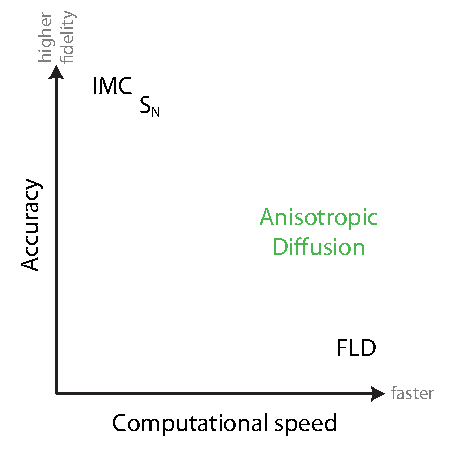
\includegraphics[width=3in]{../figures/fidelity2}
\end{center}
{\tiny
This material is based upon work supported under a National Science Foundation
Graduate Research Fellowship and a Department of Energy Nuclear Energy
University Programs Graduate Fellowship. Any opinions, findings, conclusions or
recommendations expressed in this publication are those of the author and do
not necessarily reflect the views of the National Science Foundation or the
Department of Energy Office of Nuclear Energy.}
\end{frame}

%%%%%%%%%%%%%%%%%%%%%%%%%%%%%%%%%%%%%%%%
\begin{frame}
  \frametitle{References}
\bibliographystyle{ans}
\bibliography{../SRJall}
\end{frame}
%%%%%%%%%%%%%%%%%%%%%%%%%%%%%%%%%%%%%%%%%%%%%%%%%%%%%%%%%%%%%%%%%%%%%%%%%%%

%	This material is based upon work supported under a National Science
%	Foundation Graduate Research Fellowship. Any opinions, findings, conclusions
%	or recommendations expressed in this publication are those of the author(s)
%	and do not necessarily reflect the views of the National Science
%	Foundation.  
\end{document}
